\documentclass[
	12pt,
	colorbacktitle,
	accentcolor=tud1c,
	%draft,
	%twoside,
	german,
	article
%]{tuddesign/tudexercise}
% For Draft, make Report... for whatever reason normal draft doesnt work...
]{tuddesign/tudreport}

% USEPACKAGE
% changed counter for section wise counting
\usepackage{chngcntr}
\usepackage[utf8]{inputenc}
\usepackage[T1]{fontenc}
\usepackage[ngerman]{babel}
\usepackage{graphicx}
\usepackage{subcaption}
\usepackage{listings}
\usepackage{todonotes}
\usepackage[hyphens]{url}
\usepackage{ifthen}

\counterwithin{figure}{section} 
\counterwithin{table}{section} 

\newcommand{\gcenter}[4]{
	\begin{figure}[h]
	\centering 
	\includegraphics[width=#4]{#1}
	\caption{#2}
	\label{fig:#3}
	\end{figure}
}

\newcommand{\easygcenter}[2]{
	\begin{figure}[h]
	\centering 
	\includegraphics[width=#1]{#2}
	\end{figure}
}
\newcommand{\gcenterone}[1]{
	\begin{figure}[h]
	\centering 
	\includegraphics[width=.9\textwidth]{#1}
	\end{figure}
}


\newcommand{\td}[1]{
	\todo[inline]{#1}
	}
	
%makes bold code snippets
\newcommand{\bfcode}[1]{\texttt{\textbf{#1}}}

%fixes enum labels
\renewcommand{\labelenumi}{\theenumi .}
\renewcommand{\labelenumii}{\theenumii )}


%define colors for listings		
\definecolor{javared}{rgb}{0.6,0,0} 			% for strings
\definecolor{javagreen}{rgb}{0.25,0.5,0.35}    	% comments
\definecolor{javapurple}{rgb}{0.5,0,0.35} 		% keywords
\definecolor{javadocblue}{rgb}{0.25,0.35,0.75}    % javadoc

%\settitlepicture[width=.8\textwidth]{img/mindstorm.jpg}
%\printpicturesize
\begin{document}
	
	\author{}
	\pagenumbering{arabic}	
	\title{Mindroid Workshop \\ Dokumentation}
	\subtitle{Fachgebiet Echtzeitsysteme / MAKI \\ TU Darmstadt}
	
	\maketitle	

	\section{Wichtige Funktionen}
	Hier eine kleine Übersicht über die wichtigsten Funktionen beim Programmieren der Roboter.
	
	\subsection{Fahren}
		Mögliche Eingabewerte für den $speed$-Parameter liegen zwischen 0 und 1000.
		Eine maximale Geschwindigkeit von $300$ sollte ausreichen. Niedrigere Geschwindigkeiten schonen den Akku.	
		Die Distanz wird im $distance$-Parameter immer als Kommazahl in Zentimetern (cm) angegeben (z.B.: 20cm werden als $20.0f$ angegeben)
	
		\begin{table}[htbp]
		\begin{tabular}{|p{0.2\textwidth} p{0.75\textwidth}|}
		\hline
		\textbf{Typ} & \textbf{Methode und Beschreibung} \\ \hline
		void & setMotorSpeed(int speed) \\
		& \\
		& Bestimmt die Geschwindigkeit für Fahrmethoden ohne $speed$-Parameter. \\ \hline
		void & forward() \\ 
		void & backward() \\ & \\
		& Fahren mit der von $setMotorSpeed(...)$ gesetzten Geschwindigkeit. \\ \hline
		void & driveDistanceForward(float distance) \\
		void & driveDistanceBackward(float distance) \\ & \\
		& Fahren mit der von $setMotorSpeed(...)$ gesetzten Geschwindigkeit\\ 
		& Die Distanz muss in Zentimetern angegeben werden. \\ \hline
		
		void & forward(int speed) \\ 
		void & backward(int speed)  \\ 
		void & driveDistanceForward(float distance, int speed) \\ 
		void & driveDistanceBackward(float distance, int speed) \\ 		
		& \\
		& Wie oben, nur dass der $speed$-Parameter die von $setMotorSpeed()$ gesetzte Geschwindigkeit überschreibt. Nach Beendigung des Aufrufs, wird wieder die vorher gesetzte Geschwindigkeit genutzt.\\ \hline

		void & turnLeft(int degrees) \\ 
		void & turnRight(int degrees) \\ 
		void & turnLeft(int degrees, int speed) \\ 
		void & turnRight(int degrees, int speed) \\ 
		& \\
		& Dreht den Roboter um den im $degrees$-Parameter bestimmten Wert. \\
		& Der $Speed$-Parameter verhält sich wie bei den anderen Methoden. \\ \hline
		
		void & stop() \\ 
		& \\
		& Stoppt sofort alle Motoren.	\\ \hline
		\end{tabular}
		\end{table}
		
		\newpage
	\subsection{Sensoren}
		\begin{table}[htbp]
		\begin{tabular}{|p{0.2\textwidth} p{0.75\textwidth}|}
		\hline
		\textbf{Typ} & \textbf{Methode und Beschreibung} \\ \hline
		float & getAngle() \\ 
		&\\
		& Liefert den Winkel des Gyrosensors in Grad\\ \hline
		float & getDistance() \\ 
		&\\
		& Liefert die vom Ultraschallsensor gemessene Distanz in Zentimetern\\ \hline
		
		Colors & getLeftColor() \\ 
		Colors & getRightColor() \\
		&\\
		& Liefert den Wert des Linken/Rechten Farbsensors\\ 
		& Farbwerte: Colors.BLACK, Colors.BLUE, Colors.BROWN, Colors.GREEN, \\ &Colors.RED, Colors.WHITE, Colors.YELLOW, Colors.NONE\\ \hline
		\end{tabular}
		\end{table}

	\subsection{Kommunikation}
		\begin{table}[htbp]
		\begin{tabular}{|p{0.2\textwidth} p{0.75\textwidth}|}
		\hline
		\textbf{Typ} & \textbf{Methode und Beschreibung} \\ \hline
		boolean & hasMessage() \\ 
		& Prüft ob Nachricht vorhanden ist \\ \hline
		MindroidMessage & getNextMessage() \\ 
		& Ruft nächste Nachricht ab \\ \hline		
		void & broadcastMessage(String message) \\ 
		& Sendet eine Nachricht an alle Roboter \\ \hline
		String & getRobotID() \\ 
		& Gibt den Namen des Roboters zurück. \\ \hline
		void & sendLogMessage(String logmessage) \\ 
		& Sendet eine Nachricht an den Message Server \\ \hline
		void & sendMessage(String destination, String message) \\ 
		& Sendet eine Nachricht an den $destination$-Roboter \\ \hline
		\end{tabular}
		\end{table}
		
		Um eine Nachricht zu empfangen, muss zuerst mit $hasMessage()$ überprüft werden ob eine Nachricht vorhanden ist. Liefert $hasMessage()$ true zurück, kann mit $getNextMessage()$ eine Nachricht abgerufen werden. Das Beispiel in Listing \ref{lst:msg} zeigt wie das geht.
		
		\begin{lstlisting}[captionpos=b, caption=Beispiel zum Abrufen einer Nachricht, label=lst:msg]
		if (hasMessage()){
          String msg = getNextMessage().getContent();
        }
		\end{lstlisting}
		
		$broadcastMessage(...)$ schickt eine Nachricht an alle mit dem selben Message-Server verbundenen Roboter.
		
		
		
	\newpage
	\subsection{Brick}
	\subsubsection{Display}
		\begin{table}[htbp]
		\begin{tabular}{|p{0.2\textwidth} p{0.75\textwidth}|}
		\hline
		\textbf{Typ} & \textbf{Methode und Beschreibung} \\ \hline
		void & clearDisplay() \\ 
		&\\
		& Löscht den Aktuellen Inhalt des Displays \\ \hline
		void & drawString(String text)\\			
		void & drawString(String text, int row)\\
		&\\
		& Schreibt den im $text$-Parameter gegebenen Text auf das Display.\\
		& Der Parameter $row$ bestimmt die zu beschreibende Zeile. \\
		& Wird der Parameter $row$ weggelassen, wir in die Mittlere Zeile geschrieben. \\

		\end{tabular}
		\end{table}
		
		\gcenter{img/ev3_display}{Koordinaten der Pixel des Displays des EV3\protect\footnotemark\ }{display}{.5\textwidth}
		
\footnotetext{ \url{https://services.informatik.hs-mannheim.de/~ihme/lectures/LEGO\_Files/01\_Anfaenger\_Graphisch\_EV3\_BadenBaden.pdf}		}

	\subsubsection{Buttons}
		\begin{table}[htbp]
		\begin{tabular}{|p{0.2\textwidth} p{0.75\textwidth}|}
		\hline
		\textbf{Typ} & \textbf{Methode und Beschreibung} \\ \hline
		boolean & isDownButtonClicked() \\ 
		boolean & isEnterButtonClicked() \\ 
		boolean & isLeftButtonClicked() \\ 
		boolean & isRightButtonClicked() \\ 
		boolean & isUpButtonClicked() \\ \hline
		\end{tabular}
		\end{table}
		
		Die Funktionen liefern $true$ wenn der entsprechende Button gedrückt wurde. Die Benennung der Buttons kannst du Abbildung \ref{fig:buttons} auf Seite \pageref{fig:buttons} entnehmen

		\newpage
	\subsubsection{Sound}
		\begin{table}[htbp]
		\begin{tabular}{|p{0.2\textwidth} p{0.75\textwidth}|}
		\hline
		\textbf{Typ} & \textbf{Methode und Beschreibung} \\ \hline
		void & setSoundVolume(int volume) \\ 
		void & playBeepSequenceDown() \\ 
		void & playBeepSequenceUp() \\ 
		void & playBuzzSound() \\ 
		void & playDoubleBeep() \\ 
		void & playSingleBeep() \\ \hline
		\end{tabular}
		\end{table}
		
		Der Parameter $volume$ nimmt Werte von 0 bis 10 entgegen.
	\subsubsection{LED}		
		\begin{table}[htbp]
		\begin{tabular}{|p{0.2\textwidth} p{0.75\textwidth}|}
		\hline
		\textbf{Typ} & \textbf{Methode und Beschreibung} \\ \hline
		void & setLED(int mode) \\ 
		&\\
		& Lässt die LED des EV3 im angegebenen Modus leuchten\\
		& Der Parameter $mode$ kann entweder als Ganzzahl von 0 bis 9 oder als Konstante angegeben werden. \\
		& Siehe Tabelle \ref{tab:led}\\
		\hline
		
		\end{tabular}
		\end{table}
		
		
		
		\begin{table}[htbp]
		\caption{Funktion der einzelnen Modi der LED}
		\begin{center}
		\begin{tabular}{r|l|l|l}
		
		\multicolumn{2}{c|}{\textbf{Modus (Parameter $mode$)}}   & \textbf{Farbe} & \textbf{Intervall} \\ 
		\multicolumn{1}{l|}{Wert} & Konstante &  &  \\ \hline
		0 & LED\_OFF & Aus & Aus \\ 
		1 & LED\_GREEN\_ON & Grün & Dauer \\ 
		2 & LED\_GREEN\_BLINKING & Grün & Blinken \\ 
		3 & LED\_GREEN\_FAST\_BLINKING & Grün & Schnell Blinken \\ 
		4 & LED\_YELLOW\_ON & Gelb & Dauer \\ 
		5 & LED\_YELLOW\_BLINKING & Gelb & Blinken \\ 
		6 & LED\_YELLOW\_FAST\_BLINKING & Gelb & Schnell Blinken \\ 
		7 & LED\_RED\_ON & Rot & Dauer \\ 
		8 & LED\_RED\_BLINKING & Rot & Blinken \\ 
		9 & LED\_RED\_FAST\_BLINKING & Rot & Schnell Blinken \\ 
		\end{tabular}
		\end{center}
		\label{tab:led}
		\end{table}
		
		\newpage
		\section{EV3 Tasten}
		Abbildung \ref{fig:buttons} zeigt dir wie die Tasten am EV3-Brick genannt werden. Die Enter-Taste wird zum Bestätigen genutzt, mit der Escape-Taste, geht es ein Menü zurück. 
		\gcenter{img/ev3_buttons.png}{EV3-Tastenbelegung\protect\footnotemark\ }{buttons}{.5\textwidth}
		\footnotetext{ Quelle http://www.ev3dev.org/images/ev3/labeled-buttons.png}
		
		Die Bedeutung der Tasten kannst du der folgenden Aufzählung entnehmen. 
		\begin{enumerate}
			\item \textbf{Escape / Zurück}
			\item \textbf{Up / Hoch}
			\item \textbf{Left / Links}
			\item \textbf{Enter / Bestätigen}
			\item \textbf{Right / Rechts}  
			\item \textbf{Down / Unten}  
		\end{enumerate}
	
		\section{PAN Einrichtung}
		\label{sec:pan}
		Wird im Hauptmenü noch nicht die richtige IP-Adresse angezeigt, müssen zuerst die PAN\footnote{PAN = Personal Area Network}-Einstellungen korrigiert werden.
		
		\begin{enumerate}	
			\begin{minipage}{.45\textwidth}
				\item Dazu musst du zuerst in das \textbf{PAN-Menü} des Roboters navigieren. Wechsle mit den Links-/Rechts-Tasten bis du den Menüpunkt \textbf{PAN} siehst und betätige die \textbf{Auswahltaste}.
			\end{minipage}
			\hfill
			\begin{minipage}{.45\textwidth}
				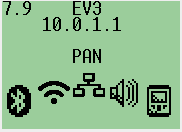
\includegraphics[width=.8\textwidth]{img/ev3_pan.png}
			\end{minipage}
			
			\item Nun navigierst du durch das Menü des Roboters wie auf den Bildern zu sehen und bestätigst jeweils mit der Auswahltaste: \textbf{USB-Client - Address - Advanced}
			
			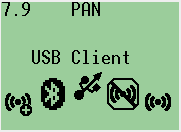
\includegraphics[width=.3\textwidth]{img/ev3_pan_usb.png}
			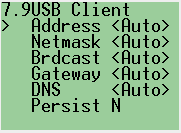
\includegraphics[width=.3\textwidth]{img/ev3_pan_usb_address.png}		
			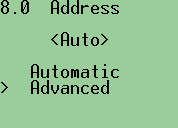
\includegraphics[width=.3\textwidth]{img/ev3_pan_usb_advanced.png}
			
			Nun musst du die IP Adresse 192.168.42.253 einstellen. Dazu navigierst du mit den rechts-/links-Tasten zu den einzelnen Ziffern und änderst deren Wert mit den oben-/unten-Tasten. Orientiere dich an den Bildern! Am Ende bestätigst du wieder mit der Enter-Taste. 
			
			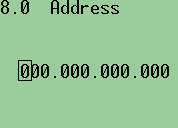
\includegraphics[width=.3\textwidth]{img/ev3_pan_usb_setip1.png}
			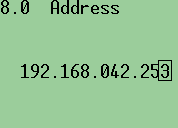
\includegraphics[width=.3\textwidth]{img/ev3_pan_usb_setip2.png}
			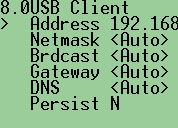
\includegraphics[width=.3\textwidth]{img/ev3_pan_usb_isset.png}
			
			\begin{minipage}{.6\textwidth}
				\item Mit der \textbf{Zurück}-Taste kommst du wieder in das Hauptmenü und die Einstellungen werden übernommen.
			\end{minipage}
			\hfill
			\begin{minipage}{.3\textwidth}
				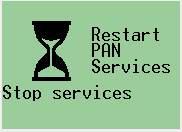
\includegraphics[width=\textwidth]{img/ev3_pan_usb_restart.png}
			\end{minipage}
			%		\\Nun kannst du wieder zu Punkt 3 auf Seite \pageref{sec:afterpan} wechseln.
		\end{enumerate}
		
		\section{Troubleshooting}
		\subsection{Installation über WLAN funktioniert nicht}
		Im Message-Server über \bfcode{File->Connected Devices }schauen ob alle Smartphones in der Liste auftauchen und der ADB-state auf \bfcode{connected} steht. 
		Ist dies nicht der Fall, tippe in der App auf \bfcode{TRENNEN} und stelle die Verbindung danach erneut her.
		Falls das nicht klappt, kontaktiere einen Betreuer. 
		Falls das Installieren per WLAN gar nicht mehr funktioniert, kann jederzeit eine USB-Verbindung zwischen Smartphone und PC hergestellt werden und darüber die App installiert werden.
		
		
		
		\section{Sensorbelegung}
		
		Tabelle	\ref{tab:sensors} zeigt die standardmäßige Sensorbelegung, wie sie in der App unter ``Mein Roboter'' definiert sein muss.
			
		Tabelle \ref{tab:motors} zeigt den standardmäßigen Motoranschluss, wie er in der App unter ``Mein Roboter'' definiert sein muss.
		
		\begin{minipage}[b]{.45\textwidth}\centering
		%	\begin{table}[htbp]
				%\begin{center}
					\begin{tabular}{r|l|l}						
						\textbf{Anschluss} & \textbf{Sensortyp} & \textbf{Modus} \\ \hline
						1 & Farbe & ColorID \\ 
						2 & Ultraschall & Distance \\ 
						3 & Gyroskop & Angle \\ 
						4 & Farbe & ColorID \\ 
					\end{tabular}
				%\end{center}
				\caption{Sensorbelegung}
				\label{tab:sensors}
		%	\end{table}	
		\end{minipage}
		\hfill
		\begin{minipage}{.45\textwidth}
			\begin{table}[htbp]
			%	\begin{center}
					\begin{tabular}{r|l}						
						\textbf{Anschluss} & \textbf{Motor} \\ \hline
						A & Large Regulated Motor \\ 
						B & - \\ 
						C & - \\ 
						D & Large Regulated Motor \\ 
					\end{tabular}
			%	\end{center}
				\caption{Motorbelegung}
				\label{tab:motors}
			\end{table}
			
		\end{minipage}
	

				
	\end{document}
